%%%%%%%%%%%%%%%%%%%%%%%%%%%%%%%%%%%%%%%%%%%%%%
%%%%%%%%%%%%%%%%%%%%%%%%%%%%%%%%%%%%%%%%%%%%%%
%%% Master Thesis Template by Fabian Schär %%%
%%%%%%%%%%%%%%%%%%%%%%%%%%%%%%%%%%%%%%%%%%%%%%
%%%%%%%%%%%%%%%%%%%%%%%%%%%%%%%%%%%%%%%%%%%%%%

%%%%%%%%%%%%%%%%%%%%%%%%%%%%%%%%%%%%%%
%%% Packages and Document Settings %%%
%%%%%%%%%%%%%%%%%%%%%%%%%%%%%%%%%%%%%%

\documentclass[12pt,a4paper,titlepage,oneside,english]{article}

%%% Main Packages %%%
\usepackage[english]{babel}
%\usepackage[ngerman]{babel} % Use this option for German settings.
\usepackage[T1]{fontenc}
\usepackage[utf8]{inputenc}

%%% Additional Packages %%%
\usepackage{cite}
\usepackage{framed}
\usepackage{graphicx}
%\usepackage[german]{fancyref}
%\usepackage[german,hidelinks]{hyperref} %hidelinks
\usepackage{multirow}
\usepackage[round]{natbib}
\usepackage{setspace}
\usepackage{geometry}
\usepackage{pst-all} % Not working with Sweave!!!
\usepackage{hyperref}

%%% Math Packages %%%
\usepackage{amsmath}
\usepackage{amstext}
\usepackage{amssymb}
\usepackage{theorem}
\usepackage{epsfig}
\usepackage{longtable}

%%% Layout Specifications %%%
\geometry{a4paper, top=35mm, left=40mm, right=40mm, bottom=45mm,
headsep=10mm, footskip=12mm}

%%% Tikz Styles %%%
\usepackage{tikz}
\usetikzlibrary{backgrounds}
\usetikzlibrary{arrows}
\usetikzlibrary{shapes,shapes.geometric,shapes.misc}

% this style is applied by default to any tikzpicture included via \tikzfig
\tikzstyle{tikzfig}=[baseline=-0.25em,scale=0.5]

% these are dummy properties used by TikZiT, but ignored by LaTex
\pgfkeys{/tikz/tikzit fill/.initial=0}
\pgfkeys{/tikz/tikzit draw/.initial=0}
\pgfkeys{/tikz/tikzit shape/.initial=0}
\pgfkeys{/tikz/tikzit category/.initial=0}

% standard layers used in .tikz files
\pgfdeclarelayer{edgelayer}
\pgfdeclarelayer{nodelayer}
\pgfsetlayers{background,edgelayer,nodelayer,main}

% style for blank nodes
\tikzstyle{none}=[inner sep=0mm]

% include a .tikz file
\newcommand{\tikzfig}[1]{%
{\tikzstyle{every picture}=[tikzfig]
\IfFileExists{#1.tikz}
  {\input{#1.tikz}}
  {%
    \IfFileExists{./figures/#1.tikz}
      {\input{./figures/#1.tikz}}
      {\tikz[baseline=-0.5em]{\node[draw=red,font=\color{red},fill=red!10!white] {\textit{#1}};}}%
  }}%
}

% the same as \tikzfig, but in a {center} environment
\newcommand{\ctikzfig}[1]{%
\begin{center}\rm
  \tikzfig{#1}
\end{center}}

% fix strange self-loops, which are PGF/TikZ default
\tikzstyle{every loop}=[]

\input{../assetlib/tikz/styles.tikzstyles}

%%% Parskip Settings %%%
\setlength{\parskip}{3mm}
\setlength{\parindent}{0mm}

%%% Document Specifications %%%
\title{A solidity smart contract for rental deposit accounts}
\author{Matthias Nadler}


%%%%%%%%%%%%%%%%%%
%%% Title Page %%%
%%%%%%%%%%%%%%%%%%

\begin{document}
%\begin{titlepage}
\begin{center}
\vspace{1em}
%\large{Seminar Paper}\\
%\large{Bachelor Thesis}\\
\large{Seminar Thesis}\\
\huge A solidity smart contract \\
for rental deposit accounts \\
\Large \vspace{1em}
Matthias Nadler
\end{center}

\vspace{1em}
\normalsize
\begin{flushleft}
Supervised by:\\ 
Prof. Dr. Fabian Schär \\
Credit Suisse Asset Management (Schweiz) Professor for \\ 
Distributed Ledger Technologies and Fintech \\
Center for Innovative Finance, University of Basel
\end{flushleft}

\vspace{1em}
\onehalfspacing
\begin{center}
\section*{Abstract}
\end{center}
TEMP: Analyze the incentive structure of the current rental deposit account situation and devise
a DAI powered smart contract that will invest the locked funds. \\
\vfill
\textbf{Keywords:} Ethereum, smart contract, DAI, rental deposit account.\\
\noindent\textbf{JEL:} G21, G52, G19
%\end{titlepage}


%%%%%%%%%%%%%%%%%%%%%%%%%%%%%%%%%%%%%%%%
%%% Inhaltsverzeichnis & Plagiatserklärung
%%%%%%%%%%%%%%%%%%%%%%%%%%%%%%%%%%%%%%%%

\pagenumbering{gobble}

\newpage
\pagenumbering{Roman}
\tableofcontents
\vfill
\begin{center}
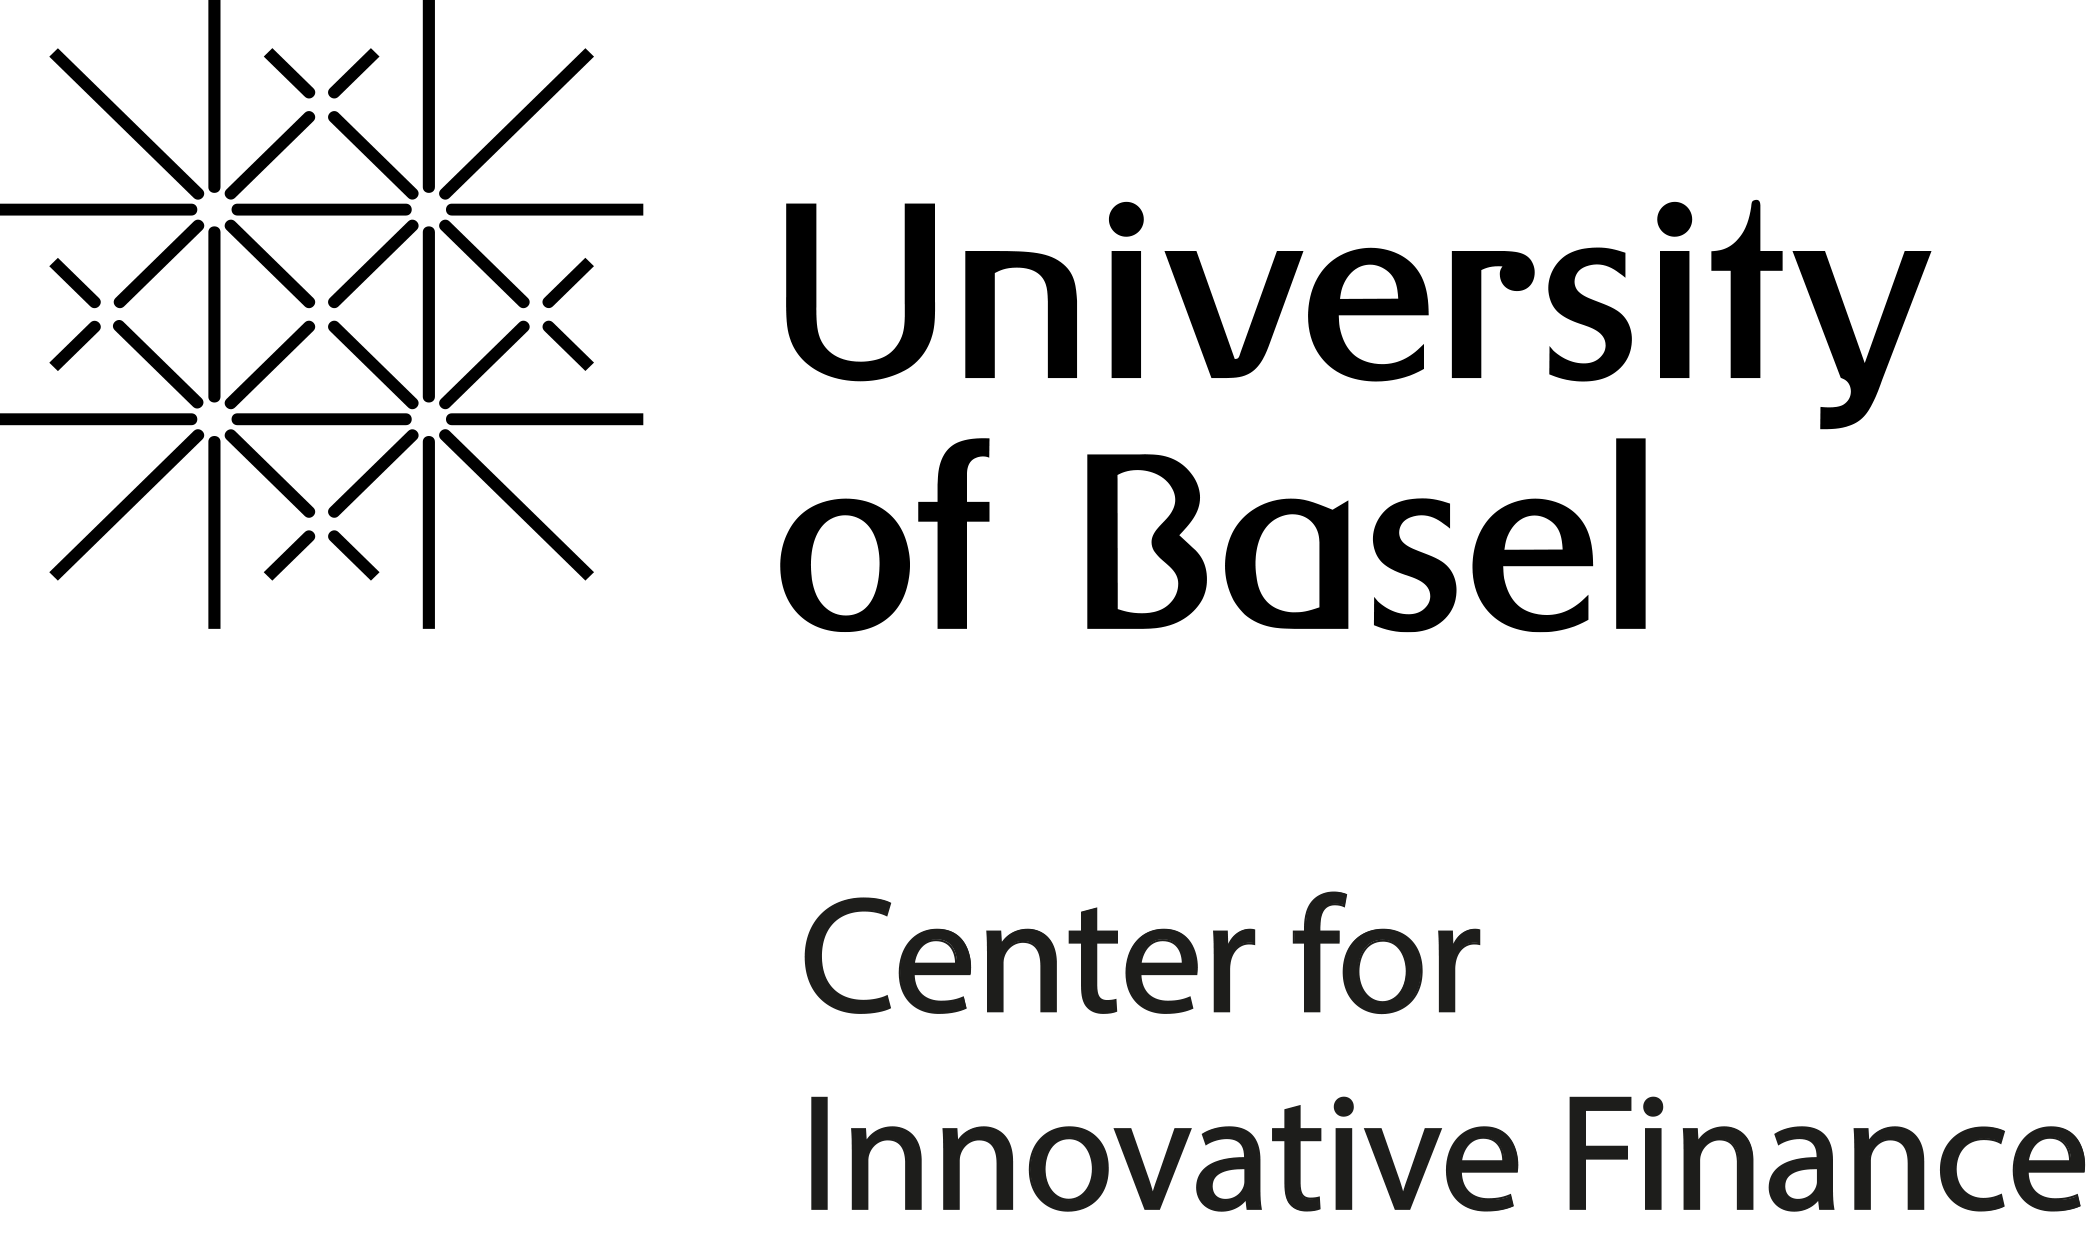
\includegraphics[width=4cm]{../assetlib/images/logo_cif.png}
\end{center}
\singlespacing
\vspace{-1.5cm}
\section*{Plagiatserklärung}
Ich bezeuge mit meiner Unterschrift, dass meine Angaben über die bei der Abfassung meiner Arbeit benutzten Hilfsmittel sowie über die mir zuteil gewordene Hilfe in jeder Hinsicht der Wahrheit entsprechen und vollständig sind. Ich habe das Merkblatt zu Plagiat und Betrug vom 22. Februar 2011 gelesen und bin mir der Konsequenzen eines solchen Handelns bewusst.\\

%% YOUR NAME HERE %%
Matthias Nadler
%%%%%%%%%%%%%%%%%%%%

\newpage
\onehalfspacing
\pagenumbering{arabic}


%%%%%%%%%%%%%%%%%%%%%%%%%%%%%%%%%%%%%%%%
%%% Introduction
%%%%%%%%%%%%%%%%%%%%%%%%%%%%%%%%%%%%%%%%

\section{Introduction}
\label{sec:introduction}
In Switzerland, according to the code of obligations (\textit{dt. Obligationenrecht, OR})  Art. 257e para. 1, a rental deposit needs to be placed in a (savings-) account at a bank, or in a deposit on the tenants name. The interest rate for a rental deposit account at one of Switzerland's largest three banks is between 0\% (UBS, Credit Suisse) and 0.05\% (Raiffeisen).\footnote{As of March 8th 2020, according to the official rates published by the banks.}

Setup, changes and release or restitution related to the deposit account all have to be handled in paper forms and require the signatures of both the tenant and the renter. These are time consuming processes for all involved parties.

The presented rental deposit account (short: RDA) smart contract attempts to solve both problems, allowing for higher interest rates for the tenant and for immediate, digital and secure transactions between the parties. 

\subsection{Smart Contracts}
\label{sub:smart-contracts}
Smart contracts are similar to traditional contracts, but they are written in a computer language and deployed on a system that is accessible to all contract parties. When interacting with a smart contract program or protocol, the code is able verify your instructions and enforce the resulting actions.

There are a few issues and questions that arise with the implementation of smart contracts. Most of these can be elegantly solved by deploying the smart contract on a public blockchain\footnote{It is assumed that the reader is familiar with blockchain and accompanying terminology. For an in-depth introduction to the topic the author recommends \cite{Schaer2017} (in German) or \cite{Lewis2018} (in English).} with a Turing complete language\footnote{A touring complete programming language has all the necessary instructions to solve any computational problem given enough resources. Bitcoin for example does not have a touring complete language, therefore no universal smart contracts can be deployed on this blockchain.}.


\begin{description}
	\item[Availability] A public blockchain is always online and accessible from everywhere. Each smart contract is deployed at a fixed address on the blockchain.
	\item[Authentication] Blockchains use private key cryptography to guarantee ownership of accounts. Smart contracts need no additional authentication logic.
	\item[Immutability] The most difficult feature to replicate without a public blockchain. The code of a deployed smart contract can never be changed. This means no one has the ability to alter the contract retroactively. Often times this also removes the need for a third party trustee and makes completely trust-less interactions possible.
	\item[Power to enforce] Smart contracts, like any other address, can directly control digital assets built on top of the blockchain. Any coin or token sent to a contract can not be recovered  unless it is transferred by the contract logic.
	\item[Transparency] The full contract code and every past interaction with the smart contract is stored on the blockchain and publicly available.
\end{description}

Our rental deposit account will combine a smart contract as described above with traditional off-chain contracts to create a more efficient agreement between the involved parties.

\subsection{Ethereum}
\label{sub:ethereum}

Any blockchain that implements a Turing complete programming language can be used to develop smart contracts. Among these options, Ethereum is the most popular according to an ecosystem report by \cite{ElectricCapital2019}: Of all open source crypto developers, 18\% worked in the Ethereum ecosystem during the first half of 2019. This is around four times more than for the second most popular platform EOS.

More reasons to develop this project on Ethereum include: The University of Basel teaches Solidity - the Ethereum specific programming language - in their courses. Ethereum has the widest array of decentralized finance products%TODO: citation
, including a very successful stablecoin which is the cornerstone of our application. Finally, the shortcomings of Ethereum compared to its alternatives - fewer transactions per second and higher transaction costs - are mitigated since our contract will perform very few transactions over its lifetime.



%%%%%%%%%%%%%%%%%%
%%% Incentives %%%
%%%%%%%%%%%%%%%%%%

\section{Improving rental deposit accounts}
In this section we will give a short overview of how a smart RDA contract operates and then take a look at the distribution of incentives, obligations and risks for each of the three parties in a traditional rental deposit account contract and how these aspects change for the smart contract variant.
It is assumed the reader is familiar on a basic level with the workings of smart contracts on the Ethereum blockchain.\footnote{Reference to more information for smart contracts and addresses}

\subsection{Smart RDA contract}
A smart RDA contract can be created by anyone for a small transaction fee. To create it, one has to specify immutable Ethereum addresses for the three involved parties: Tenant, renter (landlord) and trustee; as well as a fixed trustee fee. The tenant then transfers the full deposit amount in DAI - a crypto stablecoin\footnote{Reference to stablecoins} - to the contract and starts the contract with another transaction. This locks the DAI security in the DAI savings rate contract (short: DSR) and begins to generate compounding interest on the locked capital. Details for the DSR contract and the interest rate are described in (see section). The trustee fee is paid by the contract to the trustee using aggregated interest.
Figure \ref{fig:contract} shows a more detailed, schematic view of how the smart RDA works. Note that it is not possible to interact with the deposit directly, every action is delegated by the RDA smart contract. Actions shown with a dotted line require the consent of at least two participants before they can be executed.

\begin{figure}[h]
\ctikzfig{contract}
\caption{The smart RDA contract is in control}
\label{fig:contract}
\end{figure}

\subsection{The trustee}
The recommendation by Swiss Law (OR Art. 257e para. 1) is to store the deposit in the form of money or other securities on a (savings-) bank account. The reason for using a bank as the trustee is to minimize the counterparty risk. The bank assumes the role of a trustee and guarantees to safe-keep the deposit until it is eventually released to the tenant or renter. According to OR Art. 257e para 3., the release of the deposit can be requested in a form signed by the tenant and the renter or with a legal instruction by a court or debt enforcement office. During the lifetime of the deposit, the bank is in full control; they can invest it and keep the earnings of this investment. As noted in \hyperref[sec:introduction]{section 1}, the interest passed on to the owner of the deposit is between 0\% and 0.05\% p.a. 

The smart rental deposit account contract still requires a trustee to trigger a release of the deposit to the right party if the tenant and the renter are not in agreement. But contrary to the traditional bank deposit, the counterparty risk is greatly mitigated by using a smart contract since the control over the funds will always remain with the contract and not the trustee.
For this reason, the role of the trustee can be assumed by any entity that both the tenant and the renter can agree upon: For example a notary or an institution that offers this service. A compensation has to be provided to the trustee to perform his services, but this compensation, called a trustee fee, can be in form of a one time fixed payment.

\subsection{The tenant}
With a smart rental deposit contract the locked assets of the tenant are securely invested (while remaining under full control of the contract) and the tenant is eligible for any resulting earnings. On the other hand, the tenant has to pay the fixed trustee fee and assume all of the newly arising risks linked to the underlying technology (see section X for detailed risks). As long as the interest rate of the DSR contract is sufficiently high, the renting period is sufficiently long (to offset the trustee fee) and the tenant values the risks of a system failure low enough, the smart deposit contract will provide a significant upgrade to the traditional system for the tenant.

\subsection{The renter}
Ideally, nothing would change for the renter. However, the additional risks that arise by using a new and developing technology can not be fully absorbed by the tenant. A small risk remains for the renter: The underlying asset losing some or all of its value while the tenant at the same time becomes insolvent. 
To compensate for this, we suggest to increase the total amount of the deposit. For example use four instead of three month's worth of rent as the deposit. Note that this is much less detrimental for the tenant than it would be in a traditional setting, as the locked assets will be invested at a profit.

\subsection{Speed and ease of settlements}
Interacting with a traditional rental deposit account poses significant transaction costs for all involved parties: Every action requires a written form with the signatures of the tenant and the landlord to be sent to the bank. For the smart RDA, all these actions can be performed instantly online with a very small transaction fee (a few cents)\footnote{Note about gas costs}. If multiple signatures are needed for an action, it can only be executed once the required parties have digitally agreed on the execution. The details for this process are described in the next section. 

Authenticity of the signatures is guaranteed by the blockchain technology with the additional upside that any arbitrary document can be attached to an RDA and signed by the participants. This could for example be used to digitally sign the rental contract, eliminating the need for any physical documents and signatures in a tenant-renter relationship.


%%%%%%%%%%%%%%%%
%%% Risks    %%%
%%%%%%%%%%%%%%%%

\section{Risks}
In this section we discuss the most urgent risks that arise when using an RDA smart contract. The risks can be divided into Counterparty risk, foreign exchange risk and Layer 1 - Layer 4 risks as described by (cite DeFi paper Schär). The following sections assume that the RDA smart contract works as intended; the risk of smart contract failure is covered in Layer 3 risks.

\subsection{Counterparty risk}
As counterparty risk we understand the likelihood that one of the involved parties does not perform their contractual obligations, due to malicious intent or otherwise.
Most of the counterparty risk is mitigated by the smart contract nature of the RDA. Especially the funds are kept completely secure and can't be compromised. The obligations of the trustee - confirming multisig transactions when needed - need to be backed up by a written (off-chain) contract and there remains a risk that the trustee defaults on these obligations. However, the trustee has no personal gain from this behaviour and is contractually liable. It is still vital to chose a reputable entity for this task.

The tenant or landlord can not behave in a way that will compromise the smart contract as long as the trustee fulfils their obligation.

\subsection{Foreign exchange risk}
Currently the only widely available stablecoins on the Ethereum platform are pegged to the US-Dollar; therefore the rental deposit needs to be paid in US-Dollar. If the US-Dollar is not the local currency of the country where the RDA contract is settled, there exists a risk for the deposit to become undercollateralized if the US-Dollar is devalued. This risk can be mitigated with hedging or similar strategies if desired, otherwise the tenant and the landlord need to agree to absorb this risk. A further possibility would be to include a contract clause that will trigger a migration of the contract with re-collateralization should the exchange rate fall below a certain threshold.

\subsection{Settlement layer risk}
Layer 1 risks include a partial or total failure of the Ethereum protocol due to technical issues. This would most likely also default the entire rental deposit. The tenant is fully liable for this risk and needs to set up a new rental deposit on a different platform.

\subsection{Asset layer risk}
Layer 2 includes the assets built on the Ethereum protocol; relevant for this smart contract is the ERC-20 stablecoin DAI and by extension the MakerDAO ecosystem. MakerDAO is still very much a developing and experimental institution that brings the risk of a partial or complete failure. In most scenarios a total default can be prevented if the contract is migrated in time to a different platform on initiative of the trustee and the tenant. However, the tenant is responsible to re-collateralize the deposit. We try to keep the layer 2 risk minimal by not involving any other asset.

\subsection{Protocol layer risk}
The layer 3 risk is extensively described in Schär 2020, section 3. It consists of smart contract execution risk (coding errors and vulnerabilities), operational security (OpSec) risks and dependency risks (dependency on MakerDao and especially DSR). 
OpSec risks are negligible as there exists no admin key for the smart contract. Execution risk and dependency risk is absorbed by the tenant. One significant dependency risk is a low interest rate as defined by the DSR contract.

\subsection{Application layer risk}
The layer 4 risks arises if the parties decide to use the provided dApp at https://smartdepos.it or a similar external interface which has a chance to malfunction and submit faulty data to the RDA smart contract. Every participant bears this risk for themselves, but it is highest for the tenant as they need to send DAI transactions. The risk can be mitigated by interacting directly with the smart contract.


%%%%%%%%%%%%%%%%
%%% Multisig %%%
%%%%%%%%%%%%%%%%

\section{Multisig on Ethereum}
Multisig is the process when more than one account needs to sign a transaction before it can be executed. The Ethereum blockchain does not natively implement any multisig functionality unlike for example Bitcoin\footnote{Bitcoin's P2SH scheme (BIP16) can generate an address from any number of public keys with an additional parameter for how many signatures from these keys are needed for a transaction. This is implemented directly in the settlement layer and provides maximum security.}. Any implementation of multisig on Ethereum needs to be developed manually in a smart contract, which has been done by many different individuals and companies. However, these implementations are on the protocol layer, not the settlement layer and therefore much more open to mistakes, bugs and vulnerabilities. The famous parity hacks of 2017 - see (cite parity hacks) - were both caused by a careless implementation of the parity multisig wallet. It is therefore critical to build the multisig part of the RDA smart contract on a simple, understandable, verified and audited code base.


\subsection{Different approaches to multisig}
Signatures can be aggregated on-chain or off-chain and the content of the transaction can be stored on-chain or not. Which approach to use depends mostly on the use case of the contract.

\subsection{Off-Chain implementation}
This implementation is the closest to how Bitcoin implements their multisig: A transaction is created off-chain and then sequentially signed by the required addresses. The multi-signed transaction data is then sent to a smart contract where the signatures are verified and the transaction data executed. A standardized method to process these transactions is described in EIP191 and a minimalistic implementation by Christian Lundkvist can be found here: https://github.com/christianlundkvist/simple-multisig/blob/master/contracts/SimpleMultiSig.sol.

The main advantage of this approach is minimal mutable state on the blockchain. A transaction (and by extension assets) can't end up in a locked state where they are lost due to an invalid state of the contract. The complexity and room for bugs is also much smaller as the whole validation and execution is done in a single function call and the gas costs for the whole process are kept very low (only the account executing the transaction pays any gas).

The two main disadvantages are first, that low level non-transaction call data needs to be signed and it is not trivial, especially for more complicated transactions, for the signer to understand exactly what they are signing. And second, the signers need to coordinate off-chain in order to fully sign the transaction.

\subsection{On-Chain implementation}
On-Chain multisig stores the transaction in some form - either as direct call data or as struct of parameters - as a state on the contract. This transaction can then be signed by calling a sign function on the contract, which collects the signatures in a mapping. Once the required signatures have been collected, the transaction can be executed. A very popular and audited implementation of this method is the GNOSIS Multisig wallet which currently holds around 350'000 ETH across its most significant instances (Aragon, Golem, Myterium and District0x).

The main advantages of this approach is a complete on-chain settlement with no additional coordination between the signers and a transparent log of confirmations and executions that is permanently stored on the blockchain.

Compared to an off-chain approach, more gas is needed to complete the settlement and the increased complexity of the code renders the contract more susceptible to undesired states and vulnerabilities.

\subsection{Conclusion}
Our propsed RDA smart contract will perform a very limited number of multisig transactions over its lifetime; we can therefore disregard the slightly higher costs needed for an on-chain settlement. The transparency and persistent logs in combination with a simple coordination mechanism are however very desirable. For these reasons we pursue an on-chain approach and decided to base our implementation of multisig heavily on the proven GNOSIS multisig wallet code. A more technical overview of our implementation will be presented in (reference section).



%%%%%%%%%%%%%%%%
%%% Contract %%%
%%%%%%%%%%%%%%%%

\section{Functionality of the RDA smart contract}
The RDA smart contract is split into three different modules which are outlined in this section.
\subsection{DSR module: SavingDai.sol}
The DSR module is responsible for generating interest on the locked deposit funds.
\subsection{Core Contract with multisig: multisigRDA.sol}
core functionality
\subsection{Factory for RDA contracts: RDAregistry.sol}
factory-child with lookup


%%%%%%%%%%%%%%%%%%%%%%
%%% Implementation %%%
%%%%%%%%%%%%%%%%%%%%%%

\section{Implementation}
Software development philosophy.
\subsection{Environment}
Tools used
\subsection{Testing}
Testing approach and coverage


%%%%%%%%%%%%%%%%%%
%%% Discussion %%%
%%%%%%%%%%%%%%%%%%

\section{Discussion}
Discussion of result and potential applications


%%%%%%%%%%%%%%%%%%%%%%%%%%%%
%%% Literaturverzeichnis %%%
%%%%%%%%%%%%%%%%%%%%%%%%%%%%

\newpage
\setcounter{page}{1}
\pagenumbering{roman}
\onehalfspacing
\addcontentsline{toc}{section}{References}
\bibliography{DepositAccount}
\bibliographystyle{agsm}

%\section{Appendix}
\end{document}
